\documentclass[titlepage,11pt]{article}
\usepackage[pdftex,colorlinks]{hyperref}
\usepackage{tikz}
\usepackage{forest}
\usepackage{xcolor,graphicx,float}
\usepackage{rotating}
\usepackage{pdflscape}
\usepackage[T1]{fontenc}
\usepackage{textcomp}
\usepackage{amsmath}

\definecolor{folderbg}{RGB}{124,166,198}
\definecolor{folderborder}{RGB}{110,144,169}

\def\Size{4pt}
\tikzset{
  folder/.pic={
    \filldraw[draw=folderborder,top color=folderbg!50,bottom color=folderbg]
      (-1.05*\Size,0.2\Size+5pt) rectangle ++(.75*\Size,-0.2\Size-5pt);  
    \filldraw[draw=folderborder,top color=folderbg!50,bottom color=folderbg]
      (-1.15*\Size,-\Size) rectangle (1.15*\Size,\Size);
  }
}

\usepackage{datetime}
\newdate{date}{11}{11}{2015}

\begin{document}
\title{Aro Spot Counting Suite Tutorial}
\author{Diptodip Deb}
\begin{titlepage}
\begin{center}
\vspace*{1cm}
\huge
\textbf{Aro Spot Counting Suite Tutorial}

\vspace{0.5cm}
\Large
\textbf{For Dr. Paaby's Lab}

\vspace{1.5cm}

Diptodip Deb

\vfill

A guide for and explanation of the Aro Spot Counting Suite for use in counting cells in FISH images of worm embryos.

\vspace{0.8cm}

\large
Paaby Lab, Biology Department\\
Georgia Institute of Technology\\
\date{\displaydate{date}}

\end{center}
\end{titlepage}
\tableofcontents
\pagebreak

\section{Introduction}

This is a guide to using the Aro Suite to count cells in worm embryos. Aro was created by Scott Rifkin $<$\href{mailto:sarifkin@ucsd.edu}{sarifkin@ucsd.edu}$>$. Aro uses a machine learning approach called the Random Forest algorithm (\href{http://link.springer.com/article/10.1023\%2FA\%3A1010933404324}{Breiman, 2001}) to classify bright spots in FISH microscopy images as either cells or not cells (spots or not spots). This allows for highly accurate ($\geq$95\%) automated counts of thousands of cells across multiple worm embryos.

\section{Preparation}

In order for Aro to work, you have to do a bit of prep work. First you have to set up MATLAB to be able to use Aro, then you have to make sure your images are named and organized in a certain way, and then you have to make mask files for your images or image stacks. If you have already set up Aro in MATLAB, then skip to Section \ref{sec:imageprep}. If not, then follow the instructions below.

\subsection{A note about directories for Aro}

Aro is particular about the way that files and folders and named and set up.\\

First, you need to set up a folder for your current project. This could be something like \texttt{DataSet} for example. This folder will be referred to as the working directory or the top directory. 

Within the working directory, there should be a folder called \texttt{ImageData} that will contain the image \texttt{.stk} files. Within \texttt{ImageData}, there should be a folder called \texttt{SegmentationMasks} that contains the image mask \texttt{.tiff} files. The rest of the folders will be set up later and semi-automatically by Aro Suite. For a list of all the folders you should have at the end, see Figure \ref{fig:folders}.

\begin{figure}
\begin{forest}
  for tree={
    font=\sffamily,
    grow'=0,
    child anchor=west,
    parent anchor=south,
    anchor=west,
    calign=first,
    inner xsep=7pt,
    edge path={
      \noexpand\path [draw, \forestoption{edge}]
      (!u.south west) +(7.5pt,0) |- (.child anchor) pic {folder} \forestoption{edge label};
    },
    before typesetting nodes={
      if n=1
        {insert before={[,phantom]}}
        {}
    },
    fit=band,
    before computing xy={l=15pt},
  }
[DataSet
  [ImageData
    [dye1]
    [dye2]
    [\ldots]
    [dye\textit{n}]
  ]
  [SegmentationMasks]
  [AnalysisDir
    [Plots]
    [SegStacks
      [dye1]
      [dye2]
      [\ldots]
      [dye\textit{n}]
    ]
    [TrainingSets]
    [WormGaussianFit
      [dye1]
      [dye2]
      [\ldots]
      [dye\textit{n}]
    ]
  ]
]
\end{forest}
\caption{A folder tree showing the directory setup for using Aro.}
\label{fig:folders}
\end{figure}

\subsection{Setting up Aro in MATLAB} \label{sec:arosetup}

You'll need to set up Aro in MATLAB if you want to run it locally (as opposed to on the PACE/other compute cluster).

\begin{enumerate}
\item Download the Aro Suite from 

$<$\href{https://github.com/diptodip/AroSpotFindingSuite/archive/master.zip}{https://github.com/diptodip/AroSpotFindingSuite/archive/master.zip}$>$ if you have not already done so.
\item Extract the zip file and copy the resulting folder to \texttt{\~{}/Documents/MATLAB}.
\item Open MATLAB and on the \texttt{HOME} tab, find the \texttt{ENVIRONMENT} section. Click on \texttt{Set Path} (see Figure \ref{fig:aroinstall}).
\item In the dialogue box that pops up, click on \texttt{Add With Subfolders}.
\item Navigate to \texttt{\~{}/Documents} and select the \texttt{\~{}/MATLAB} folder that has the Aro Suite folder inside. Then hit \texttt{Open}.
\item Hit Save. Ignore any warnings about saving \texttt{pathdef.m} and needing administrator rights and just hit OK to all of them.
\end{enumerate}

\begin{figure}
\centering
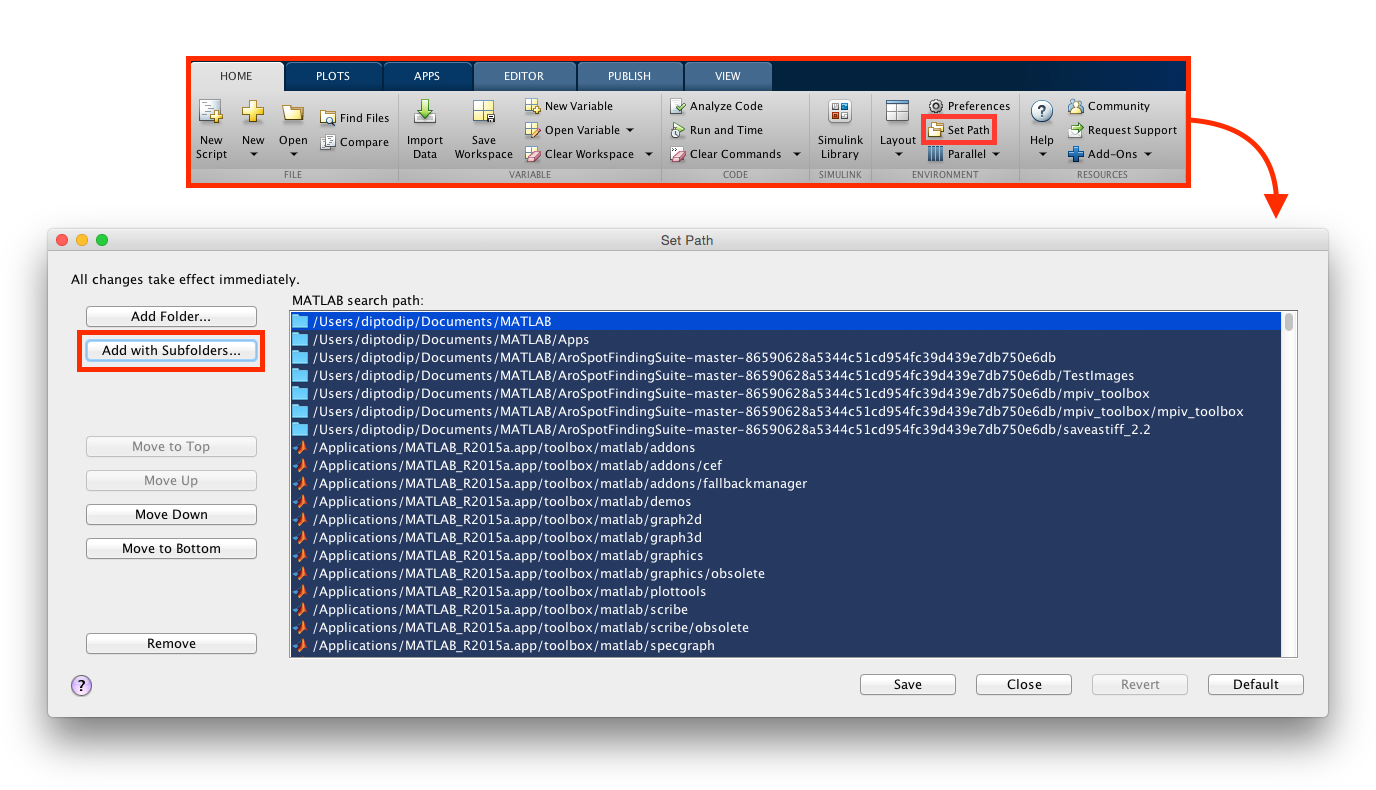
\includegraphics[scale=1.45]{aroinstall.png}
\caption{Screenshots that show how to set up the Aro files in MATLAB.}
\label{fig:aroinstall}
\end{figure}

\subsection{Prepare your image files} \label{sec:imageprep}

Aro is also very picky about the way that your image files are named and organized --- but it has to be. This is how it knows which files are which and when to use which file. If you mess up your file naming, you could throw off the whole set of counts. Be careful!

\begin{enumerate}
\item In your working directory, make a folder called \texttt{ImageData} if you haven't already.
\item For each image file, place the file in the \texttt{ImageData} folder with the filename formatted as \texttt{dye\_xxx.stk} where \texttt{dye} is the name of the \texttt{dye} and \texttt{xxx} is the 3 digit position number (e.g. position 1 is 001). Possible image formats include \texttt{.stk} and \texttt{.tiff} files.
\end{enumerate}

\subsection{Prepare masks for your images} \label{sec:maskprep}


In order for Aro to be able to identify distinct embryos you must provide mask images. You will make a separate mask image for each embryo in an image stack file. Each mask image will become a position later. This step will become more clear after following the instructions once through.\\

Note that we can automatically produce mask images with the command \texttt{auto\_trim\_mask\_directory}. This command will both automatically trim the stacks in your image directory to the frames that show the embryo and produce a mask image for the embryo in the appropriate location. You can review these masks with the command \texttt{show\_mask\_preview} as long as you are in the top level directory (i.e. the directory containing the \texttt{SegmentationMasks} folder).

\begin{figure}
\centering
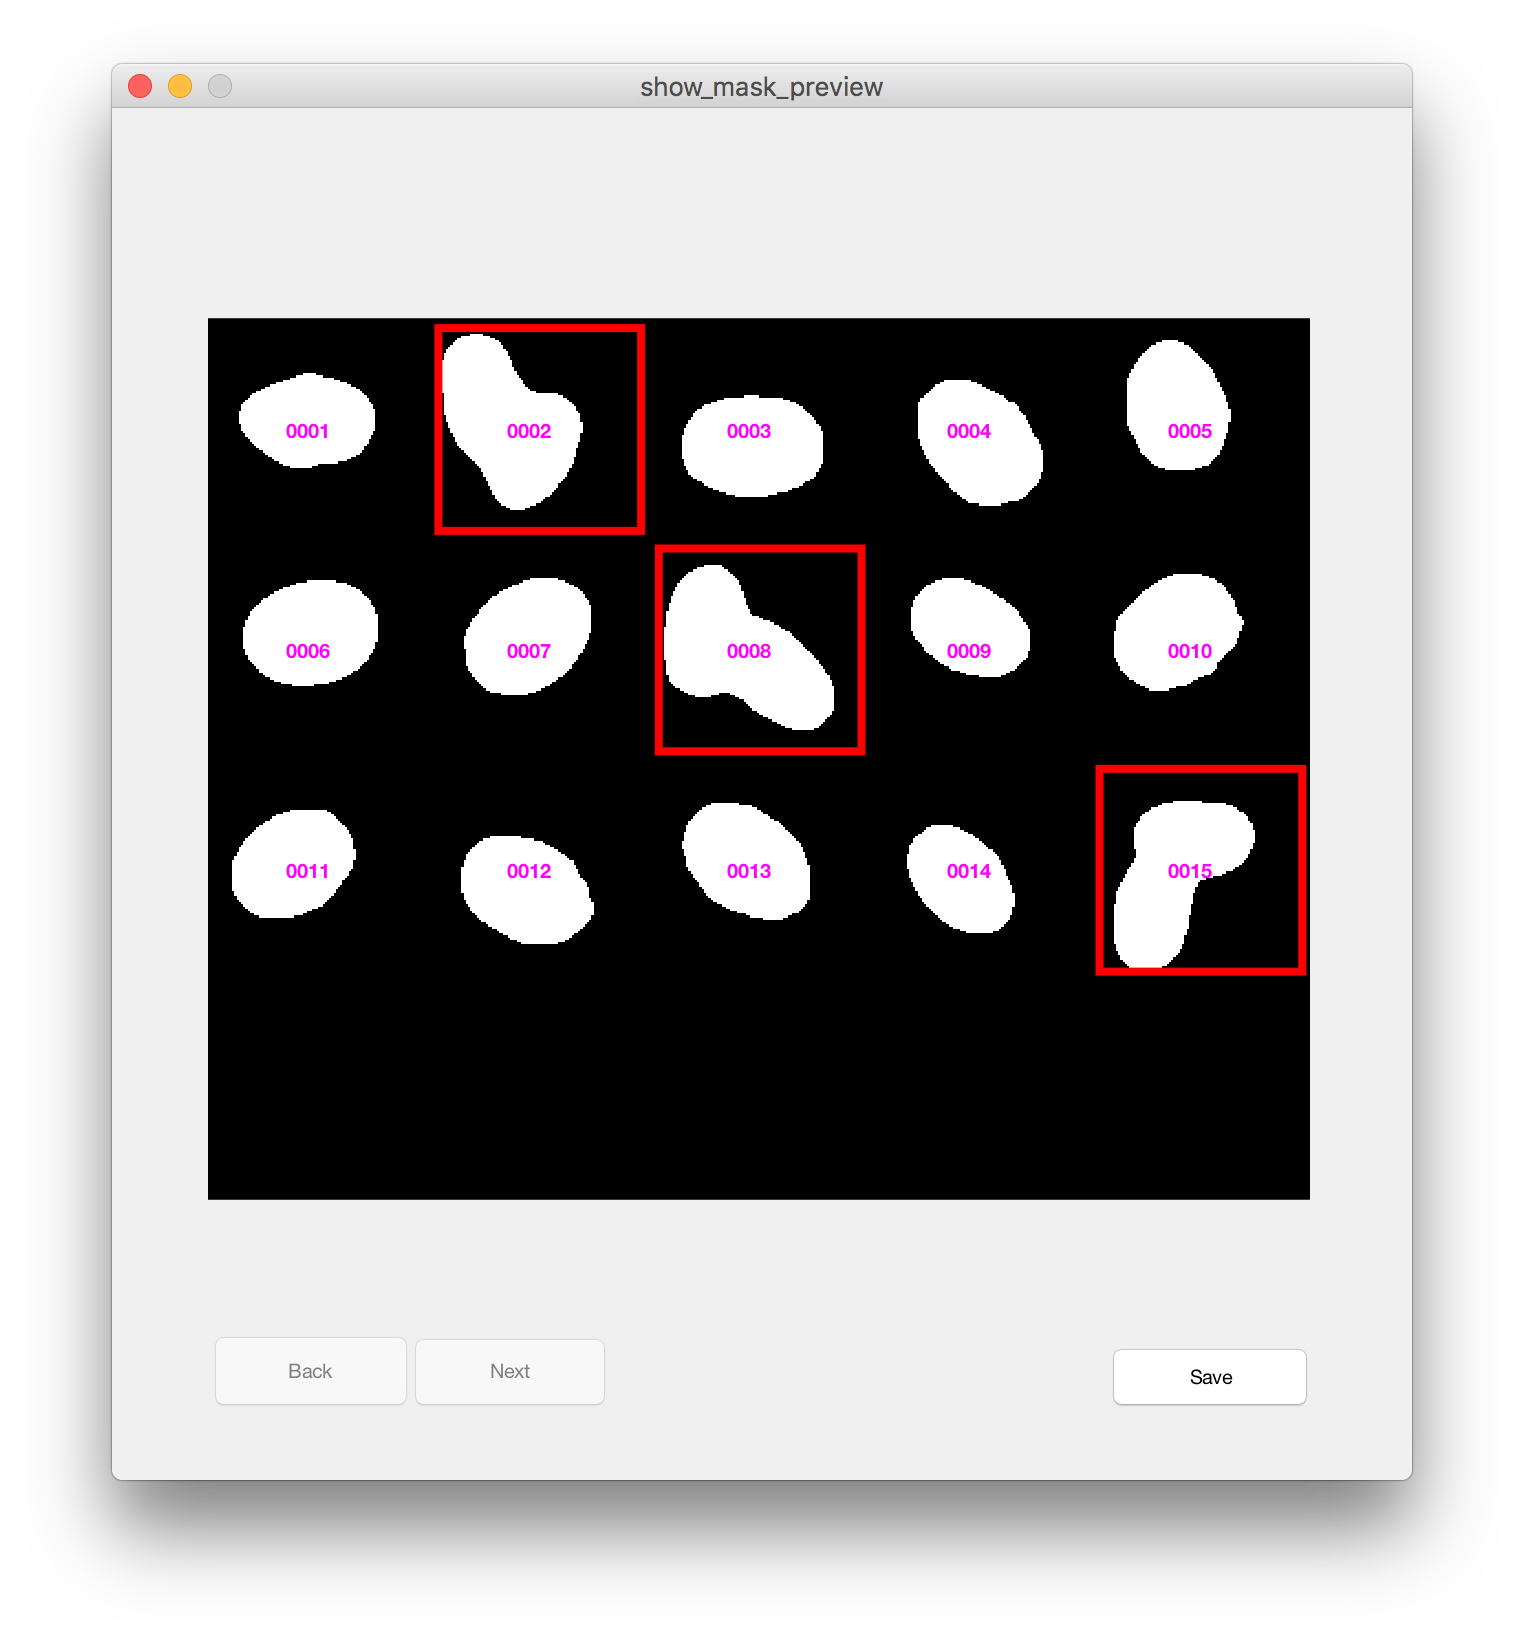
\includegraphics[scale=0.45]{show_mask_preview.png}
\caption{Screenshot showing the GUI for previewing the mask files. The red boxes indicate masks that have been determined to be bad masks. Aro will automatically run a check for predicting bad masks, but this will not find all bad masks/find false positive bad masks. Clicking a thumbnail will toggle the status of the mask file. Files with bad masks will not be analyzed.}
\label{fig:showmaskpreview}
\end{figure}

Howeever, we can also make masks manually. In order to make the mask images, we will use ImageJ. For macOS, you can find instructions on how to install ImageJ on their website at $<$\href{http://imagej.nih.gov/ij/docs/install/osx.html}{http://imagej.nih.gov/ij/docs/install/osx.html}$>$.

\begin{enumerate}
\item Open your stack file in ImageJ.
\item Select one of the embryos using the "Freehand selections" tool.
\begin{itemize}
\item See Figure \ref{fig:masks}.
\item Make sure you are in the middle of the stack.
\item Make sure you do this with a steady hand.
\end{itemize}
\item In the menu, go to \texttt{Edit > Selection > Create Mask}.
\item In the menu, go to \texttt{Edit > Invert}.
\item Save the mask as a \texttt{.tiff} file by going to \texttt{File > Save As > Tiff...}
\begin{itemize}
\item Make sure you name the file in the format: \texttt{Mask\_xxx\_y.tiff} where \texttt{xxx} is the 3 digit position number and \texttt{y} is the single digit mask number, e.g. \texttt{Mask\_001\_1.tiff} is the first mask for the first image (so it is the mask for the first embryo in the position 001 stack). All the mask files should be placed under the \texttt{ImageData/SegmentationMasks} folder.
\end{itemize}
\end{enumerate}

\subsection{Set up a parameter file for your data set}

Now that your image folders are set up, you need to create a file that tells Aro where the files that it will look for are located. Keep in mind the folder structure shown in Figure \ref{fig:folders}.

\begin{enumerate}
\item In your working directory, place a copy of the \texttt{example-parameters.m} file that came with your copy of Aro.
\item Rename that file to \texttt{Aro\_parameters.m}.
\item In MATLAB, open up this new parameters file.
\item Make sure that the \texttt{nestedOrFlatDirectoryStructure} option is set to equal \texttt{\textquotesingle nested\textquotesingle}.
\item Set the \texttt{dyesUsed} variable to be a cell array of strings representing the names of your dyes, i.e. \texttt{dyesUsed=\string{\textquotesingle dye1\textquotesingle,\ldots, \textquotesingle dye\textit{n}\textquotesingle \string};} and e.g. \texttt{dyesUsed=\string{\textquotesingle cy\textquotesingle,\textquotesingle tmr\textquotesingle \string};}.
\item Set the \texttt{AnalysisDir} variable to equal a string representing the name of the Analysis folder, e.g. \texttt{Analysis\_ddMonthyy}.
\item Keep everything else the same.
\end{enumerate}

\begin{landscape}
\begin{figure}
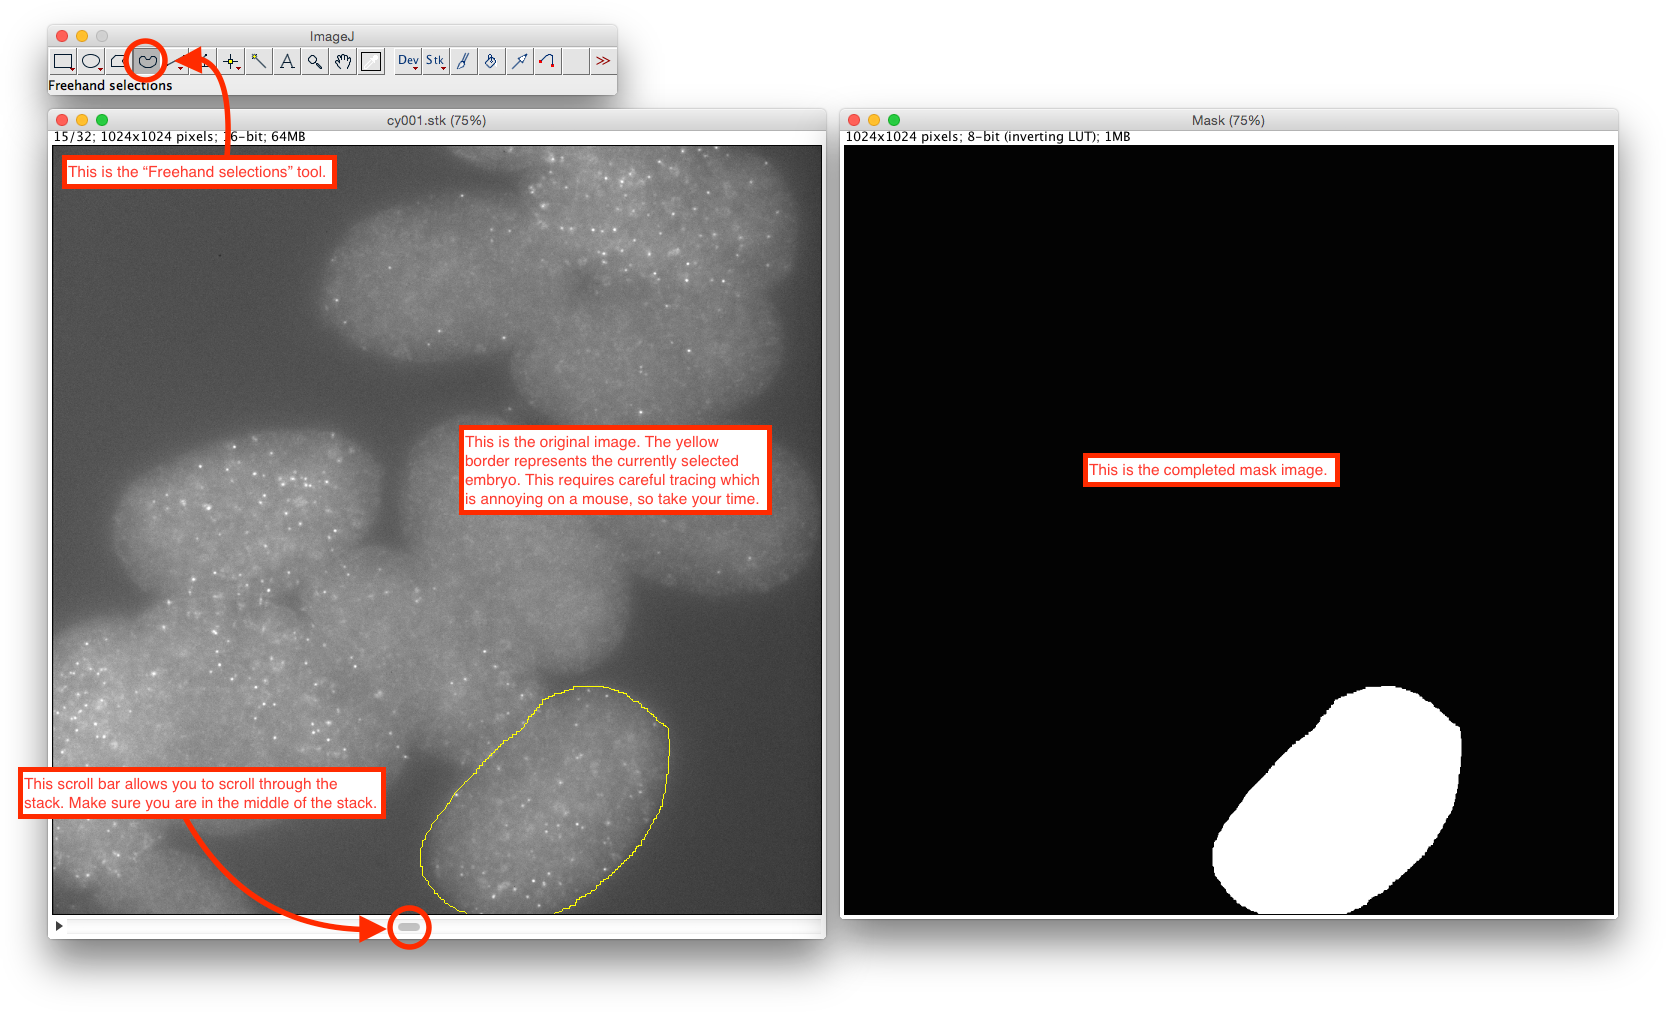
\includegraphics[scale=1.6]{masks.png}
\caption{Screenshots showing the creation of a mask from a FISH image in ImageJ.}
\label{fig:masks}
\end{figure}
\end{landscape}

\subsection{Create segmentation masks for Aro}\label{sec:createsegmasks}

After creating the mask files for all the images of embryos at all the positions, you need to run an Aro command that allows Aro to understand the mask files. This is a distinct step from the previous step in which we made masks for the images. Note that you \textbf{do not} need to do this if you have used the command \texttt{auto\_trim\_mask\_directory} to produce the masks.\\

From the top directory, open MATLAB and in the command window run \texttt{createSegmenttrans(\textquotesingle Posx\textquotesingle)} if you want to process just the mask file for position x or \texttt{createSegImages(\textquotesingle tif\textquotesingle)} if you want to process all the mask files in the \texttt{SegmentationMasks} directory.

Each command will create a \texttt{dye\_xxx\_segStacks.mat} file that tells Aro where the embryos are for each dye and each position. By this point, the naming scheme should be obvious.

\section{Classifying Spots With Aro}

Now Aro should be ready to go with your data set. Settle in, this will be the longest part of the counting process.

\subsection{Find candidate spots for each cell}

In this step, Aro will find local brightness maxima for each image and make some (for now) black box calculations to describe each local maximum.\\

This will allow Aro to make guesses at which parts of the images could be spots to be counted. These guesses will become the candidate spots. This process is designed to include all possible spots regardless of whether or not each candidate is a real spot or not.

This process will create files of the form \texttt{dye\_xxx\_wormGaussianFit.mat} for each position and each dye. These files contain the stats for the candidate spots. These files will be saved in the \texttt{WormGaussianFit} folder.

In order to find candidate spots for all embryos, run the command \texttt{doEvalFISHStacksForALL} from your working directory.

\subsection{Use Aro to classify the spot candidates}\label{sec:classification}

Aro uses the Random Forest algorithm to calculate the number of spots in each embryo. In order to do this, it has to first make a training set in order to learn what a spot looks like in each dye (dye is also referred to as color channel). Then, using what it has learned from the training set, Aro classifies each of the candidate spots in the images as either a spot or not a spot in order to output a count of the number of spots in each embryo in each image (position).

\subsubsection{Create a training set}\label{sec:trainingsets}

The Random Forest algorithm needs user input to make the training set, i.e. the user has to give Aro examples of which spot candidates are actually spots. Some important guidelines to follow: 
\begin{itemize}
\item Images between different data sets and even different dyes within the same data set can look very different. Make a new training set for each data set and each dye.
\item In fact, Aro can't use training sets from one data set for another data set without producing errors later on, so don't reuse training sets.
\item Good training sets will have both positive and negative examples, i.e. good examples of spot candidates that are spots and spot candidates that are not spots. Try to include as many positive examples as negative examples and also throw in a few ambiguous (in-between) examples that are hard even for a human to classify.
\item Don't start right off with a huge set of training data. It's better to train with a few spots, observe the performance, and then make corrections and add those to the training set. Doing three or four rounds of this should be enough, and a training set that starts with around 300-400 spots for the first round of training is recommended.
\end{itemize}

\begin{enumerate}
\item From the working directory, run the MATLAB command 

\texttt{createSpotTrainingSet(\textquotesingle dye\_Posx\textquotesingle,\textquotesingle Probe\_name\textquotesingle)}.
\item In the \texttt{identifySpots} GUI window that pops up, either accept or reject spots (see Figure \ref{fig:identifySpotsGUI}).
\begin{itemize}
\item Keep the guidelines above in mind.
\item Especially remember to train spots across slices.
\item Do \emph{not} touch the \texttt{Spot Rank} slider.
\end{itemize}
\item When finished, hit the \texttt{Done} button to close the \texttt{identifySpots}.
\item When \texttt{Finished} is pressed, a dialogue box will pop up asking if you want to continue training. Select \texttt{No}.
\item There should now be a \texttt{trainingSet\_dye\_Probe\_name.mat} file in the \texttt{TrainingSets} folder.
\end{enumerate}

\begin{landscape}
\begin{figure}
\centering
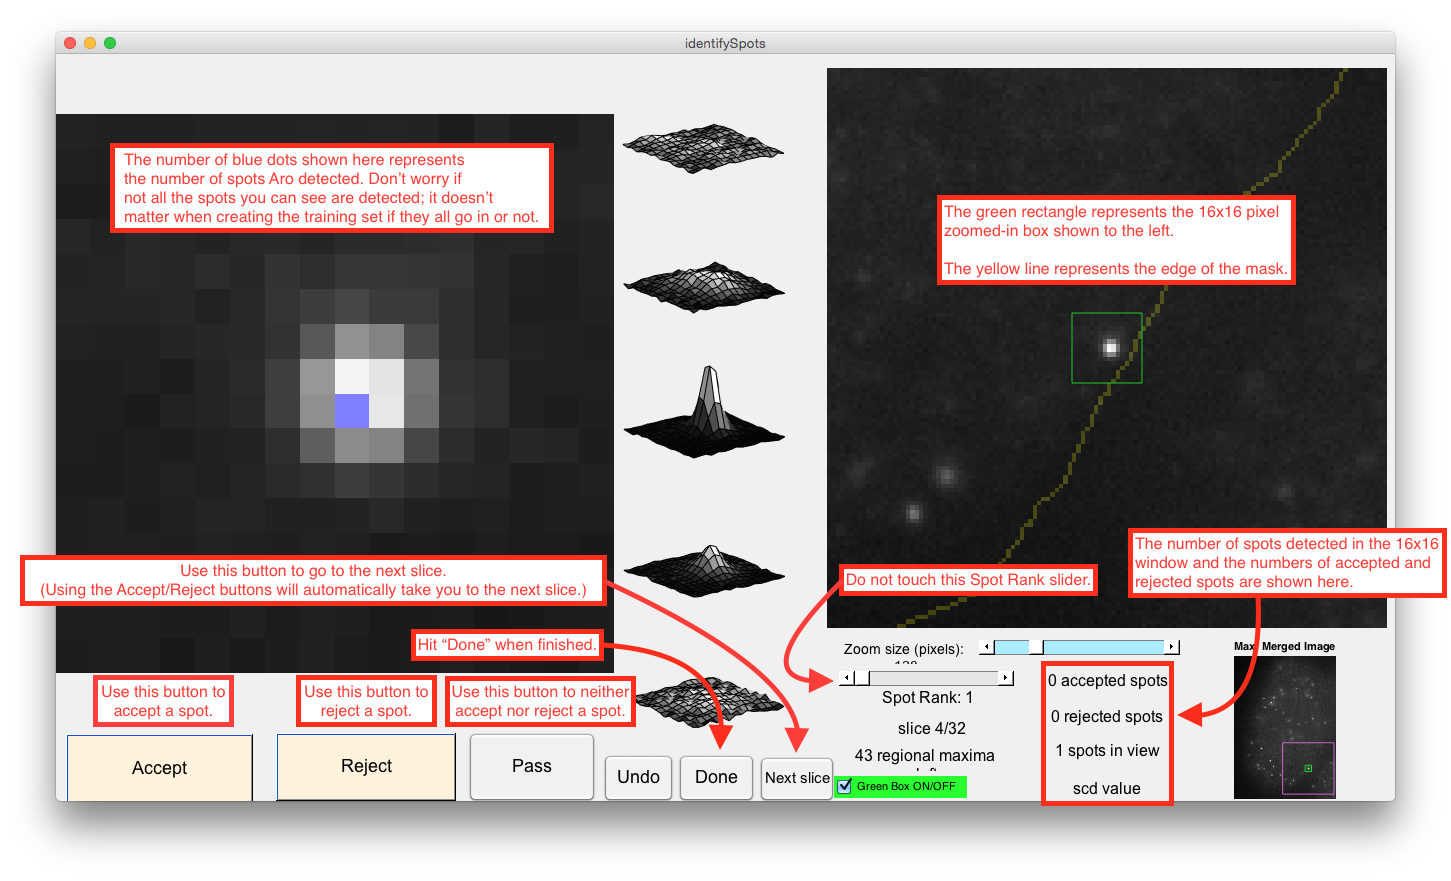
\includegraphics[scale=0.4]{identifySpotsGUI.png}
\caption{A labelled screenshot of the identifySpots GUI.}
\label{fig:identifySpotsGUI}
\end{figure}
\end{landscape}

\subsubsection{Use the training set to train a classifier}
Now that a training set has been created, it can be used to train a classifier. The classifier is the part of Aro that, given a training set and a set of data about worms (remember the \texttt{wormGaussianFit.mat} file), will classify candidate spots as spots or not spots.

\begin{enumerate}
\item From the working directory, run the MATLAB command 

\texttt{load trainingSet\_dye\_Probe\_name.mat} where dye is the name of a dye and Probe\_name is the name of a probe.
\item From the working directory, run the MATLAB command 

\texttt{trainingSet=trainRFClassifier(trainingSet)}.
\begin{itemize}
\item Don't be alarmed if this step takes a while. If you had 1000 training spots (you won't the first time), for example, this step could take 5 - 30 minutes depending on processing power.
\item At the end of this process, you should have an updated \texttt{trainingSet} file and a new \texttt{dye\_Probe\_name\_RF.mat} file that contains the random forest data. The random forest data will also be in the updated \texttt{trainingSet} file.
\item Remember, these files will be in the \texttt{TrainingSets} folder (see Figure \ref{fig:folders}).
\end{itemize}
\item Repeat these steps until there is a training set for every dye.
\end{enumerate}

\subsubsection{Classify the spots using a training set}
After a training set has been made, it can be used for an initial classification of the spots of a particular dye and probe. Don't expect this to be too accurate. Later, you will review this classification and make corrections to improve the training set and, by extension, the classifier.

\begin{enumerate}
\item From the working directory, run the MATLAB command 

\texttt{load trainingSet\_dye\_Probe\_name.mat}. This naming scheme should be obvious by now.
\item In your MATLAB Workspace, you should see the variable \texttt{worms} and \texttt{trainingSet}.
\item From the working directory, run the MATLAB command
\texttt{classifySpotsOnDirectory}.
\begin{itemize}
\item You could also choose to classify only a specific dye and specific position by using the command 
\texttt{classifySpots(worms, trainingSet)}. In order to run this command you would have to first run the commands
\texttt{load trainingSet\_dye\_Probe\_name.mat} and
 
\texttt{load dye\_Posx\_wormGaussianFit.mat}.
\item Another option is to still use \texttt{classifySpotsOnDirectory} but specify a training set and a dye. In order to do this, first load in the appropriate training set using the command given above. Then, from the working directory run the MATLAB command
\texttt{classifySpotsOnDirectory(toOverWrite, trainingSet, dye)}. The parameter \texttt{toOverWrite} is a numeric boolean (1 or 0) that specifies whether the files should be overwritten or not and should of course be set to 1 to have the command do anything useful.
\item It is recommended that instead of using specifics you just run the generic 
\texttt{classifySpotsOnDirectory} command. This will automatically classify all the spots for all the appropriate dyes and training sets for all the positions for you, which is what you want when you are reviewing the classification later.
\end{itemize}
\end{enumerate}

\subsubsection{Review the classified spots and retrain}
Use the \texttt{reviewFISHClassification.mat} GUI to review the spots classified by Aro. This step corrects classification errors made by Aro and gives you the option to add the corrections back to the training set. Don't try to correct all the errors at once --- do three or four rounds of corrections.\\

\begin{enumerate}
\item From the working directory, run the MATLAB command 

\texttt{reviewFISHClassification(dye\_Posx)}.
\item In the GUI window that opens, make corrections to the classifications (see Figure \ref{fig:reviewFISHClassificationGUI}). If this is the first review, don't expect the classification to be very accurate.
\begin{itemize}
\item Make sure that you are adding your corrections to the training set.
\item Make as many corrections as possible, but don't try to fix everything.
\item Remember to keep the guidelines for picking good training spots in mind.
\end{itemize}
\item When finished, press the \texttt{All Done} button. This will pop up a dialogue box asking "Retrain the classifier now?" to which you should respond by pressing the \texttt{Yes} button.
\begin{itemize}
\item This process can take a while (remember how long training took the first time --- there are even more spots now). \emph{Do not close if it looks like it's not doing anything! Check the MATLAB Command Window --- it is probably still running the training step.}
\item You can also retrain without pressing \texttt{All Done} as shown in Figure \ref{fig:reviewFISHClassificationGUI}, but this is not recommended because it will probably just slow you down unnecessarily (you should be redoing and rechecking the classification after each retraining anyway). 
\end{itemize}
\item Repeat this process until the classifier does not appear to show improvement (approximately 3 - 4 times).
\item Repeat the retraining procedure for all the classifiers (i.e. each dye/probe). Try to use multiple positions when retraining.
\end{enumerate}

\begin{landscape}
\begin{figure}
\begin{center}
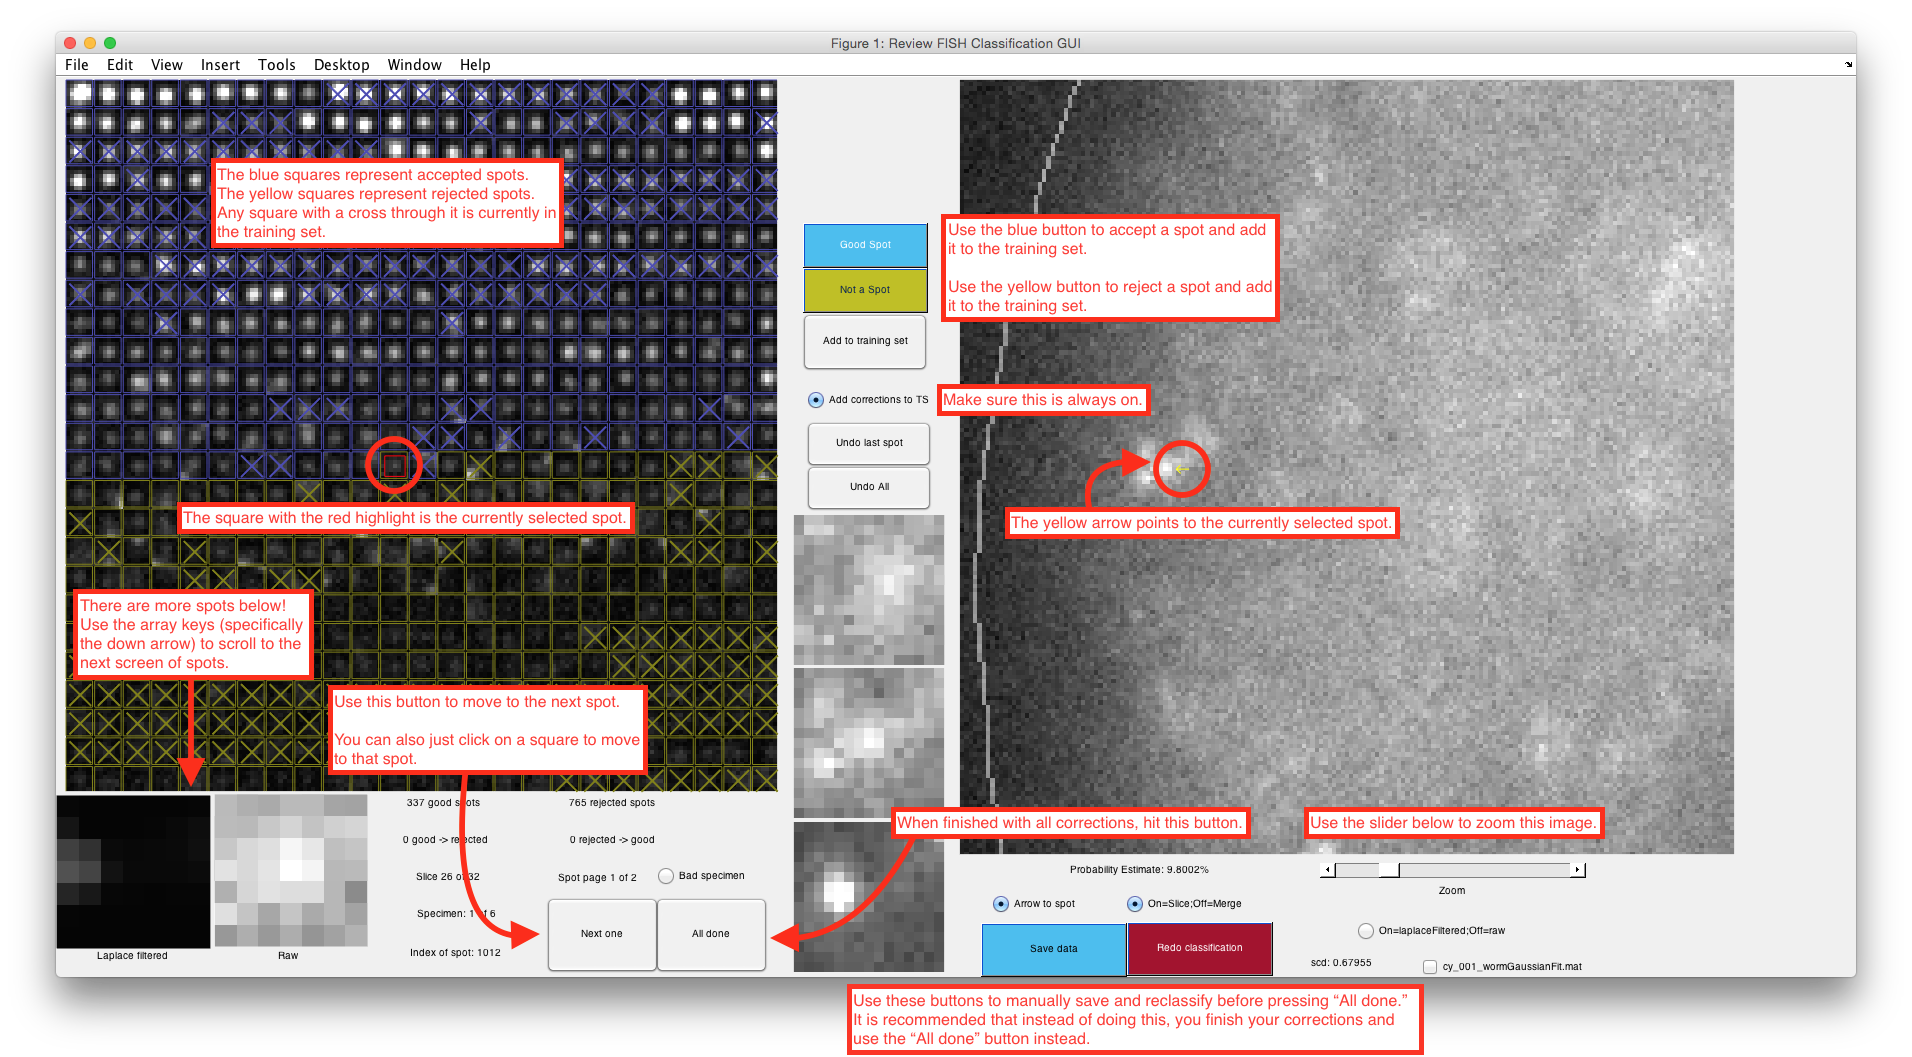
\includegraphics[scale=0.35]{reviewFISHClassificationGUI.png}
\end{center}
\caption{A labelled screenshot of the review GUI.}
\label{fig:reviewFISHClassificationGUI}
\end{figure} 
\end{landscape}

\subsubsection{Classify all spots automatically}
Once the classifiers have been sufficiently trained and retrained, it is time to let Aro count all the spots. Remember, each classifier is for one type of dye in the same data set, simply different positions.

\begin{enumerate}
\item From the working directory, run the MATLAB command \texttt{classifySpotsOnDirectory.}
\item All the candidate spots for all the embryos should now be classified.
\item Check to make sure there are newly updated \texttt{spotStats.mat} files for all the possible positions for all the dyes in the \texttt{SpotStats} folder.
\end{enumerate}

\subsubsection{Sum all the spot counts}

Aro now has the spot counts for each embryo at each position for all the dyes used. This step will give a summary of all the spot count data.

\begin{enumerate}
\item From the working directory, run the MATLAB command 

\texttt{spotStatsDataAligning2(suffix)}.
\begin{itemize}
\item The parameter \texttt{suffix} is an arbitrary file suffix that will be used to name the resulting file of this command.
\item It is recommended that the suffix be a date in the form of a string of integers, i.e. \texttt{yyyymmdd} and e.g. \texttt{20151031}.
\end{itemize}
\item This command should produce two files: \texttt{wormData\_suffix.mat} located in the \texttt{AnalysisDir} folder and \texttt{ErrorPercentagePlot\_suffix.fig} located in the \texttt{Plots} folder. For a reminder about the directory structure, see Figure \ref{fig:folders}.
\end{enumerate}

\section{Reading Results From Aro}

By now, the counting should be completed. You can now run some commands to access the completed counts data.\\

\subsection{Statistics for each position}

For any position, you can manually open up the \texttt{spotStats} file by using the MATLAB command \texttt{load dye\_Posx\_spotStats}. This will allow you to run the command \texttt{spotStats\string{\textit{n}\string}} which will display output similar to Figure \ref{fig:spotStatsOutput}.

\begin{figure}
\begin{center}
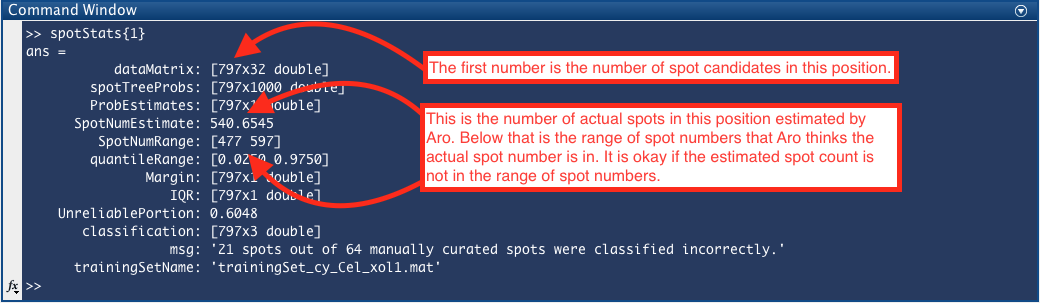
\includegraphics[scale = 0.45]{spotStatsOutput.png}
\caption{A labelled screenshot of the output from a \texttt{spotStats} file for a specific dye and position.}
\label{fig:spotStatsOutput}
\end{center}
\end{figure}

\subsection{Using the summarized data file} \label{sec:datasummary}

However, you should have already run the command \texttt{spotStatsDataAligning2}. This means there is a \texttt{wormData} file that contains summaries of relevant data for each worm and each object at each position (which should mean each embryo at each position for all the dyes used). In order to access this file, from the working directory run the MATLAB command \texttt{load wormData\_suffix}. Now, there is a MATLAB struct array with fields \texttt{spotInfo}, \texttt{dye}, \texttt{dye1}, \ldots, \texttt{dyen}, \texttt{errorPercentage}, and \texttt{meanRange} in the Workspace.

The field \texttt{spotInfo} contains information about each object (which should be each embryo --- regardless of the dyes used, since each dye should have each object for all positions). For each object, \texttt{spotInfo} contains three numbers that represent, in order: the overall number (index) of the object, the position that the object is located in, and the number (index) of the spot \emph{in that position}. Running the MATLAB command \texttt{wormData(1).spotInfo} will return a matrix containing these three values for all the objects, but this can be overwhelming when there are hundreds of embryos. Running \texttt{wormData(1).spotInfo(\textit{n},:)} will show the spot information for the $n^{\text{th}}$ object.

The field \texttt{dye} contains a list of the dyes used as defined in \texttt{Aro\_parameters.m}. The other fields that are named by each specific dye contain information about the spot counts for each of those dyes. In one of those fields, the following numbers can be found for each object (which should be each embryo): the number of the position in which the object is located, the estimated spot count for that object, the upper error, and the lower error. Running the MATLAB command \texttt{wormData(1).dye\textit{n}} will return a matrix containing these four values for all the objects. This can be overwhelming if there are a large number of embryos (just like the \texttt{spotInfo} field but there is even more data since each dye has its own field). Running \texttt{wormData(1).spotInfo(\textit{n},:)} will show the spot count estimate and other data for the $n^{\text{th}}$ object.

The field \texttt{errorPercentage} contains the error percentage of the spot estimate for each object and each dye. This value is calculated as 

\begin{equation}
\frac{\frac{U + L}{2}}{\textrm{total spot number}}\cdot100\%.
\end{equation}

\noindent$U$ represents the upper error and $L$ represents the lower error. In order to get the error percentage for the $n^{\text{th}}$ dye and $k^{\text{th}}$ object, run the MATLAB command \texttt{wormData(\textit{n}).errorPercentage(\textit{k})}.

The field \texttt{meanRange} contains the average of the difference between the upper and lower bound spot estimates (the average range) from all the objects for each dye. In order to get the mean range for the $n^{\text{th}}$ dye, run the MATLAB command \texttt{wormData(\textit{n}).meanRange}.

With each of these fields and their corresponding commands, you can access the spot count data for each embryo. It is also possible to load and view this data using the MATLAB GUI by just loading the \texttt{.mat} file in MATLAB through its file browser and viewing the variable from the MATLAB Workspace. However, once you get used to it, it will be faster to just run the commands. See Figure \ref{fig:wormDataOutput} for examples of the outputs from each of these fields.

\begin{figure}[H]
\centering
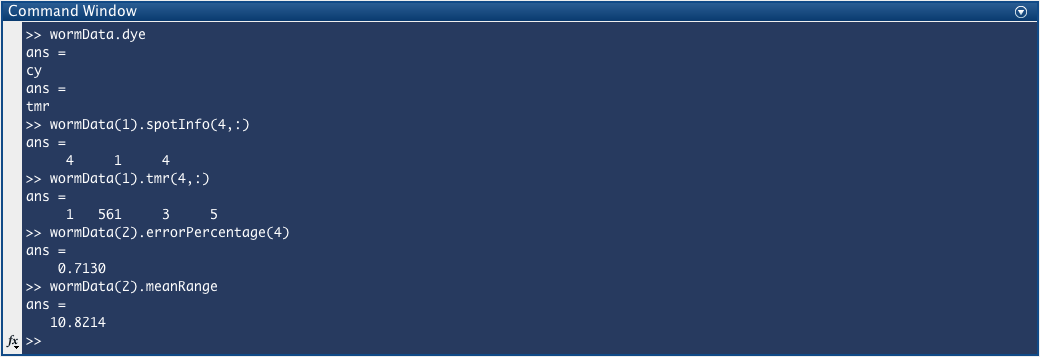
\includegraphics[scale=0.42]{wormDataOutput}
\caption{A screenshot showing example output from the various fields in \texttt{wormData} using the fourth object and the second dye.}
\label{fig:wormDataOutput}
\end{figure}

\subsection{Accessing and interpreting error plots}

When the \texttt{spotStatsDataAligning2} command was run, it produced a \texttt{.fig} file. This file is a plot of the error percentages that can be found in the \texttt{wormData} file (see Section \ref{sec:datasummary}). The plot shows error percentage versus number of spots for each object in each dye, color coded by dye. In order to view the figure, from the working directory in MATLAB, run the command \texttt{open AnalysisDir/Plots/ErrorPercentagePlot\_suffix.fig}. This will open up the plot in a MATLAB figure window. See Figure \ref{fig:errorPercentagePlot} for an example of what to expect from this plot. When the classifiers are well trained, you should see that the error percentage plot changes from a higher average error percentage to a lower error percentage for any given object. This means a poorly trained classifier will have a more globular, scattered error percentage plot while a well trained classifier will have a more flat, clustered error percentage plot. A well trained classifier also has lower mean ranges (found in \texttt{wormData(\textit{n}).meanRange}). These plots are of course not directly showing you that accuracy is improving since Aro has no idea what the proper counts actually are. However, both the error percentage plot and the mean range values should give you an idea of whether the classifier is becoming stronger.

\begin{figure}[H]
\centering
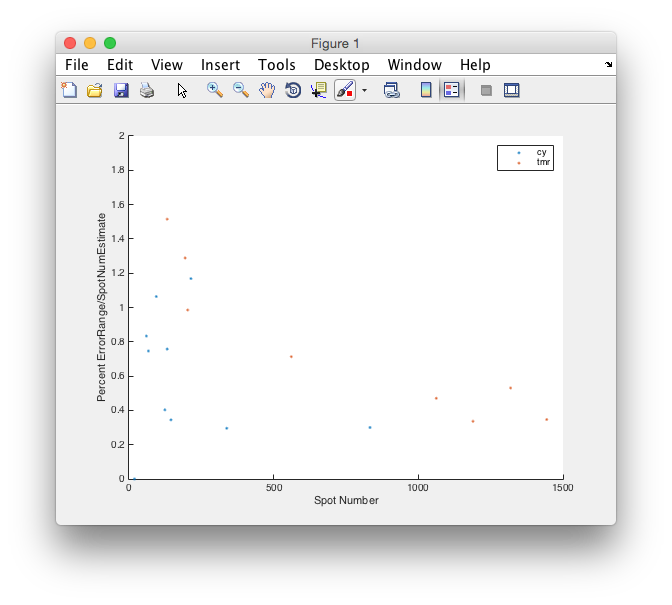
\includegraphics[scale=0.40]{errorPercentagePlot.png}
\caption{A screenshot of an error plot produced with example data.}
\label{fig:errorPercentagePlot}
\end{figure}

\section{Automatically running Aro on PACE} \label{sec:paceguide}

In order to use Aro on PACE, follow the steps below. This assumes that a training set has already been produced according to the instructions in Section \ref{sec:trainingsets}. We also assume basic knowledge of \texttt{bash} commands.
\begin{enumerate}
\item First, \texttt{SSH} into PACE using \texttt{user@biocluster-6.pace.gatech.edu}.
\item In your \texttt{data} folder, place a copy of Aro using \texttt{scp -r AroSpotFindingSuite user@biocluster-6.pace.gatech.edu:~/data/} from your local machine (this assumes you have already obtained a copy of Aro from $<$\href{https://github.com/diptodip/AroSpotFindingSuite/archive/master.zip}{https://github.com/diptodip/AroSpotFindingSuite/archive/master.zip}$>$ and that you are currently in the folder containing the Aro folder).
\item In your \texttt{data} folder, construct a new Aro project folder as detailed in Figure \ref{fig:folders}. To do this, use the \texttt{mkdir} command. Place all of the \texttt{*.pbs} script files in the Aro folder in this project folder using \texttt{cp}.
\item Copy over the \texttt{Aro\_parameters.m} example file from the Aro folder (and make sure that it is filled out properly for your analysis).
\item Submit the Aro job to the cluster queue by using \texttt{qsub full\_run\_aro.pbs}.
    \subitem Alternatively, run the steps only up to masking and producing thumbnails using \texttt{qsub automask\_pace.pbs}.
    \subitem Then, copy over the \texttt{SegmentationMasks} folder (as well as \texttt{Aro\_parameters.m}) to your local machine using \texttt{scp -r user@biocluster-6.pace.gatech.edu:~/data/<project\_folder>/SegmentationMasks ./} on your local machine (this will place the folder in your current folder on your local machine).
    \subitem Open MATLAB to the directory containing the \texttt{SegmentationMasks} folder and run the command \texttt{show\_mask\_preview} to preview the masks as shown in Figure \ref{fig:showmaskpreview}.
    \subitem Back on PACE, finish the remainder of the analysis using \texttt{qsub analysis\_after\_masks.pbs}.
\item The output of the analysis will show up as \texttt{output.csv} and the Aro log/console output will be recorded in the \texttt{*.output} file.
\end{enumerate}

\newpage
\noindent
\begin{center}
\large{\textbf{This concludes the Aro guide.}}
\end{center}

\iffalse
\newpage
\section{Appendix}

\begin{appendix}

\section{Random Forest Algorithm}

Aro uses the random forest algorithm to classify spots. The following is a brief explanation of how this algorithm works. For more details, see \href{http://link.springer.com/article/10.1023\%2FA\%3A1010933404324}{Random Forests} by Leo Breiman, 2001.

Classification is one of the fundamental problems in the field of machine learning. Generally, the machine (referred to as the classifier agent) is trained on a set of data with given classifications based on certain chosen characteristics. Once the agent receives enough training data (i.e. already classified data or data that some user classifies for the agent during the training process), the agent applies its classifer to a new set of unclassified data. Essentially, the agent is making a statistical "best guess" as to what types of characteristics lead to what classifications. Thus, when it encounters new, unclassified data, it determines the relevant characteristics of the data and makes its probable best guess using its trained classifier.

\section{MATLAB Basics}

MATLAB subsection goes here.

\section{Notes on Aro}

Aro subsection goes here.

\end{appendix}

\fi

\end{document}
